\documentclass[paper=a4,fontsize=12pt,parskip=half]{scrartcl}

%% packages
\usepackage[ngerman]{babel}
\usepackage{fontspec}
\usepackage{lmodern}
\usepackage{color}
\usepackage{graphicx}
\usepackage[autostyle=true,german=quotes]{csquotes}
\usepackage[hidelinks=true,colorlinks=false]{hyperref}
\usepackage{listings}
\usepackage[export]{adjustbox} % For frames with includegraphics
\usepackage{pgfgantt}

\definecolor{darkgray}{rgb}{.2,.2,.2}

\lstset{basicstyle=\footnotesize\ttfamily,breaklines=true}

\lstdefinelanguage{Grammar}{
  keywords={grammar, typedef, node, prop, terminal, children},
  keywordstyle=\color{blue},
  ndkeywords={string, boolean, between, allowed, sequence},
  ndkeywordstyle=\color{black},
  identifierstyle=\color{black},
  sensitive=false,
  commentstyle=\color{purple}\ttfamily,
  stringstyle=\color{red}\ttfamily,
  morestring=[b]',
  morestring=[b]"
}

\hypersetup{
  pdftitle={Generierung von syntaxfreien Programmierumgebungen für beliebige Programmiersprachen},
  pdfsubject={Bewerbung um einen Stipendienplatz},
  pdfauthor={Marcus Riemer}
}

\usepackage[backend=biber,defernumbers=true,sorting=none]{biblatex}
\addbibresource[datatype=bibtex]{diss.bib}

\begin{document}

\section*{Generierung von syntaxfreien Editoren für beliebige Programmiersprachen}

Konventionelle Entwicklungsumgebungen sind speziell auf die Bedürfnisse von professionellen Anwendern zugeschnittene Programme welche sich, aufgrund der damit verbundenen Komplexität, aus didaktischer Sicht nur eingeschränkt für die Einführung in die Programmierung eignen. Im Rahmen der Promotion soll erforscht und praktisch demonstriert werden, wie sich aus formalen Beschreibung von Programmiersprachen benutzerfreundliche, syntaxfreie Editoren speziell für Lernende erzeugen lassen können.

Abbildung~\ref{fig:example-sql-ide} zeigt ein prototypisches Beispiel für einen solchen generierten Editor. Die Konzeption dieser generierten Editoren orientiert sich an den Erfahrungen, welche die Forscher hinter Projekten wie Scratch \cite{resnick_scratch:_2009} oder Googles Blockly gemacht haben \cite{fraser_ten_2015}.

\begin{figure}[p]
  \includegraphics[width=\linewidth]{screenshot-drag-drop-ide.png}
  \caption{Generierte Umgebung für die Programmiersprache \texttt{SQL}}
  \label{fig:example-sql-ide}
\end{figure}

\lstinputlisting[float=p,label={lst:partial-sql-grammar},caption={Auszug aus der Grammatik für SQL},captionpos=b,language={Grammar}]{sql.grammar}

Bei den als Eingabe fungierenden formalen Beschreibungen handelt es sich um eine noch nicht endgültig spezifizierte Abwandlung \enquote{typischer} Grammatiken wie sie zur Definition der Syntax in fast jedem Compiler zum Einsatz kommen \cite[S. 42ff]{aho_compilers:_2007}. Dabei sind Ergänzungen und Abwandlungen notwendig, da die gängige rein syntax-orientierte Sichtweise für die Übersetzung in eine grafische Oberfläche keinerlei Informationen über die Darstellung enthält. Listing~\ref{lst:partial-sql-grammar} illustriert die Struktur dieser Grammatiken anhand eines Auszuges aus einer Grammatik für \texttt{SQL}. Die in Abbildung~\ref{fig:example-sql-ide} zu sehenden Farbstile wurden auf Basis von Eigenschaften wie \texttt{"keyword"} vergeben.

Die automatisierte Übersetzung der Grammatiken ermöglicht es erfahrenen Anwendern, zum Beispiel Lehrkräften, gegebene Programmiersprachen didaktisch motiviert einzuschränken. So wäre es zum Beispiel mögliche eine \texttt{SQL}-Variante zu erstellen, bei welcher die \texttt{GROUP BY}-Komponente nicht zur Verfügung steht. In Anlehnung an die bei \cite{klaeren_macht_2007} beschriebenen \enquote{Sprachebenen} soll sich so der Funktionsumfang der generierten Entwicklungsumgebungen an den Lernfortschritt der Klassengemeinschaft anpassen lassen.

Die automatisch generierten Editoren sollen zudem kontextsensitive Unterstützung beim Programmieren anbieten. Da alle Manipulationen durch den Benutzer immer auf einem Syntaxbaum stattfinden, können auch bei unvollständigen (Teil-)Programmen typisierte Löcher (entlehnt aus Sprachen wie Haskell \cite{jones_haskell_2014}) genutzt werden, um die Menge an verfügbaren Operationen zu limitieren oder bestimmte Operationen hervorzuheben.

Zusammengefasst sollen also folgende Aspekte erforscht und demonstriert werden, ...

\begin{itemize}
\item wie auf Basis der beschriebenen Verfahren Editoren für unterschiedliche Klassen von Programmiersprachen (z.B. \texttt{SQL}, \texttt{HTML}, \texttt{CSS}, JavaScript, ...) generieren lassen.
\item welche zusätzlichen Annotationen für Grammatiken sinnvoll und notwendig sind, um mit den generierten Oberflächen Lernenden einen möglichst intuitiven Zugang zur Programmierung zu ermöglichen.
\item wie sich für Lernende automatisiert kontextabhängige Hinweise zur korrekten Vervollständigung der Programme geben lassen können.
\end{itemize}


\section{Detaillierte Konzeption}

Ein zentraler Aspekt dieses Promotionsvorhabens liegt in der ausgewogenen Berücksichtigung von theoretischen und praktischen Anteilen: Die im Rahmen der Arbeit zu treffenden Annahmen sollen durch die praktische Implementierung bestmöglich verifiziert werden. Das Projekt befindet sich damit in einem etwas ungewöhnlichen Spannungsfeld zwischen der klassischen Informatik-Kerndisziplin \enquote{Übersetzerkonstruktion} (\enquote{Compilerbau}) und der Informatik-Didaktik. Darüber hinaus spielen auch Aspekte der Mensch-Computer-Interaktion eine Rolle, schließlich geht es neben der Verifikation der Programme auch um die Konstruktion benutzerfreundlicher Schnittstellen.

\subsection{Syntaxfreie Programmiersprachen}

Bei syntaxfreien Programmiersprachen muss der Programmierer sich nicht mit den syntaktischen Details der verwendeten Programmiersprache beschäftigen. Aus seiner Sicht spielt es keine Rolle ob z.B. Anweisungen durch Semicoli getrennt werden, Blöcke mit geschweiften Klammer, \texttt{begin} und \texttt{end} oder durch Leerraum definiert werden oder welche Klammern notwendig sind.

In der Praxis handelt es sich bei solchen syntaxfreien Sprachen de facto immer um visuelle Programmiersprachen. Auch die schon erwähnten Umgebungen Scratch und Blockly fallen in diese Kategorie. In diesen Umgebungen arbeitet der Programmierer mit der Maus um die verschiedenen zur Verfügung stehenden Blöcke an semantisch sinnvollen Orten zu platzieren. Diese Art der Programmierung ist für erfahrene Programmierer oder umfangreiche Softwareprojekte erfahrungsgemäß hinderlich \cite[S. 262f]{schiffer_visuelle_2001}, eignet sich aber zur Einführung in die Programmierung \cite{resnick_scratch:_2009}.

\subsection{Prior Art: Master-Thesis}

Die Masterthesis \enquote{BlattWerkzeug} \cite{riemer_blattwerkzeug_2016}  wurde im Oktober 2016 vom Bewerber Marcus Riemer fertiggestellt und beschreibt zwei konkrete syntaxfreie Editoren für \texttt{SQL} und \texttt{HTML}. Diese Arbeit legt in ideeller Weise den Grundstein für das Promotionsvorhaben und demonstrierte, dass sich eine Entwicklungsumgebung für Schüler prinzipiell auch von nur einem Entwickler umsetzen ließe. Im Februar 2018 wurde jedoch der gesamte Code für diese konkreten Editoren entfernt und durch einen Prototypen des hier beschriebenen neuen, generativen Ansatzes ersetzt \cite{riemer_commit_2018}.

Von der ursprünglichen Thesis bleibt damit die Idee und die grundlegende Konzeption einer einsteigerfreundlichen Entwicklungsumgebung, sowie einige generelle Erkenntnisse über mögliche Strategien zur Umsetzung. Dieses Promotionsvorhaben versteht sich als eine Iteration des ursprünglichen Ansatzes: Anstatt jede weitere zu unterstützende Programmiersprache mühsam von Grund auf neu zu entwerfen, soll die Integration weiterer Sprachen mit etablierten Techniken und Vorgehensweisen aus der normalen Übersetzerkonstruktion vorgenommen werden können.

\subsection{Eingrenzung und Wahl des Forschungsvorhabens}

Es handelt sich bei diesem Promotionsvorhaben, trotz der möglichen praktischen Anwendungen in der Informatik-Lehre, ausdrücklich nicht um eine didaktische Arbeit. Es findet folglich keine didaktische fundierte Konzeption von möglichen Lehrinhalten oder Unterrichtsstunden statt.

Diese Einschränkung ist zum Einen durch den fachlichen Hintergrund der Beteiligten bedingt: Dr. Frank Huch als Erstgutachter und Betreuer ist Informatiker und arbeitet an der CAU Kiel im Fachbereich \enquote{Übersetzerkonstruktion}. Der Promotionsstudent Marcus Riemer ist ebenfalls Informatiker und arbeitet als wissenschaftlicher Mitarbeiter an der Fachhochschule Wedel. Beiden gemein ist das Anliegen, eine möglichst frühe und effektive Vermittlung von Informatik-Kenntnissen an Schulen möglich zu machen:

\begin{itemize}
\item Dr. Huch ist an der CAU Kiel in die Ausbildung der Lehramtsstudierenden mit Fachrichtung Informatik involviert.
\item Herr Riemer ist seit seiner eigenen Schulzeit auf freiwilliger Basis für unterschiedlichste Informatik-Lehrprojekte tätig geworden.
\end{itemize}

Auch wenn es Ihrer Einschätzung nach möglich wäre, aufbauend auf der Masterthesis eine vornehmlich didaktische Arbeit zu schreiben, würde dies eine umfangreiche Einarbeitung in die entsprechenden didaktischen Hintergründe und Methoden voraussetzen. Diese Einarbeitungzeit entfällt durch die Fokussierung auf Fragestellungen und Themen aus der Informatik.

Zum Anderen halten Dr. Huch und Herr Riemer die grundlegendere Arbeit, also die automatische Erzeugung von benutzerfreundlichen Editoren, für wissenschaftlich und praktisch relevanter. Unserem Wissensstand nach existiert noch keine Software, welche die Vorgehensweise aus der Übersetzerkonstruktion zur Generierung von syntaxfreien Editoren verwendet. Und auch diese Software könnte natürlich von Leuten mit didaktischem Hintergrund erforscht werden. Es ist durchaus geplant die zu erstellende Software von z.B. Lehramtsstudierenden der CAU Kiel oder im Rahmen von Lehrerfortbildungen auf ihre Eignung für den Unterrichtsgebrauch zu prüfen.

\subsection{Technische Konzeption}

Um die einfachste Verwendung der Software für Lernende zu gewährleisten, wird der praktische Teil des Projekts als Webanwendung entwickelt. Für die ersten Schritte der Softwareentwicklung reicht auf Seiten der Lernenden dann ein beliebiger, aktueller Browser. Mit diesem Ansatz ist das Vorhaben in guter Gesellschaft: Das \enquote{große Vorbild} Scratch ist ebenfalls über den Browser erreichbar, genau so wie auch mit Blockly erzeugte Umgebungen \cite[vgl. S. 28]{riemer_blattwerkzeug_2016}.

\begin{figure}
  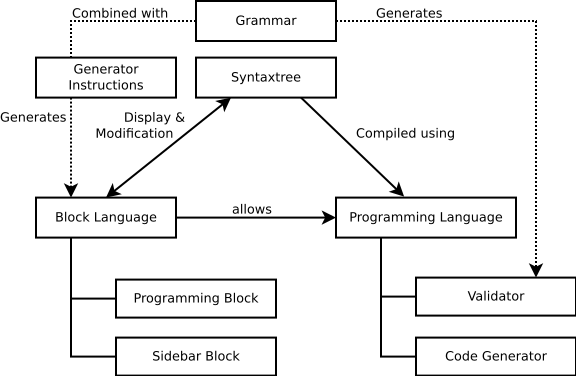
\includegraphics[width=\linewidth]{core-concepts.pdf}
  \caption{Zusammenhänge der zentralen Ressourcen}
  \label{fig:core-relations}
\end{figure}

Abbildung~\ref{fig:core-relations} veranschaulicht zentrale Begriffe des Vorhabens und deren Zusammenhänge. Auf der obersten Ebene sind beim Editieren eines Programms mit einem syntaxfreien Block-Editor (siehe Abbildung~\ref{fig:example-sql-ide} für ein Beispiel) vier grundlegende Datenstrukturen involviert:

\begin{itemize}
\item Die \textbf{Grammatik} (Grammar) definiert die grundsätzlich zulässigen Strukturen eines abstrakten Syntaxbaums. Aus dieser Beschreibung lassen sich Blocksprachen und Validatoren erzeugen.
\item Der \textbf{abstrakte Syntaxbaum} (Syntaxtree, AST) repräsentiert die Struktur eines Quelltextes der mit einem Blockeditor bearbeitet wird. In einer konventionellen Entwicklungsumgebung würde man an dieser Stelle von einer \enquote{Datei} sprechen.
\item Der Blockeditor weiß wie die zu bearbeitende \enquote{Datei}, also ein Syntaxbaum, darzustellen ist, weil er auf die Angaben in einer \textbf{Blocksprache} (Block Language) zurückgreifen kann. Diese definiert wie die einzelnen Teile des Syntaxbaumes visualisiert und editiert werden sollen und welche Blöcke verfügbar sein sollten.
\item Die tatsächliche Kompilierung und Validierung erfolgt anhand einer \textbf{Programmiersprache} (Programming Language).
\end{itemize}

Für normale Nutzer, also vornehmlich Lernende, sind diese Unterscheidungen nicht von Bedeutung. Aus Ihrer Sicht interagieren Sie im Browser mit einer Art Dateibaum und bekommen automatisch, passend zum Typ der \enquote{Datei}, entsprechende Editoren präsentiert.

Darüber hinaus kann durch die konsequente Verwendung eines abstrakten Syntaxbaumes der für andere Compiler typische Parsing-Vorgang entfallen. Anwender sollen Programme mit den generierten syntaxfreien Editoren erstellen und editieren, nicht in einem Texteditor. Die eigentliche Aufgabe der generierten Oberfläche ist somit die Bearbeitung von Syntaxbäumen.

\subsubsection{Der abstrakte Syntaxbaum}

Der Syntaxbaum als solcher ist nichts weiter als eine Datenstruktur auf der Operationen zur Veränderung (einfügen, löschen, tauschen, ...) definiert sind. Der Baum als solcher verfügt explizit über keinerlei Funktionalität zur eigenen Validierung oder zur Erzeugung von Programmcode. Er fungiert stattdessen als Eingabe für andere Module, welche diese Funktionalität bereitstellen.

Jeder Knoten eines Baums entspricht mindestens einem Typen, welcher sich aus den Strings \texttt{language} (im Sinne einer Programmiersprache) und \texttt{name} zusammensetzt. Anhand dieses Typs entscheiden alle anderen Module wie genau mit dem Knoten zu verfahren ist. Durch die Aufteilung des Typen in einen lokalen Namen und einen Namensraum (die Programmiersprache) lassen sich Namenskollisionen vermeiden:

\begin{itemize}
\item Programmiersprachen ermöglichen die Wahl von alternativen Ausführungspfaden  über bedingte Verzweigungen, welche typischerweise über das Schlüsselwort \texttt{if} zur Verfügung gestellt werden. Anhand des Sprachnamensraums können unterschiedliche Sprachen wie z.B. Ruby (in welcher \texttt{if} ein Ausdruck ist) und C (in welcher \texttt{if} eine Anweisung ist) ihr jeweiliges Konzept von Verzweigungen unter dem gleichen Bezeichner \texttt{if} definieren (\texttt{c.if} und \texttt{ruby.if}).
\item Textauszeichnungssprachen haben üblicherweise eine Möglichkeit \enquote{Überschriften} auszuzeichnen. Durch den Namensraum können alle diese Sprachen (z.B. \texttt{HTML}, Markdown oder \LaTeX) problemlos den Typnamen \texttt{Heading} verwenden ohne das es zu Mehrdeutigkeiten kommt.
\end{itemize}

\begin{figure}[p]
  \centering\includegraphics{ast-example-null.pdf}
  \caption{Syntaxbaum für \texttt{null}-Werte in einer nicht näher beschriebenen Sprache \texttt{lang}. Dieser Knoten enthält außer seinem Namen keine Daten.}
  \label{fig:ast-example-null}
\end{figure}

\begin{figure}[p]
  \centering\includegraphics{ast-example-expr-variable.pdf}
  \caption{Baum für den Einsatz einer Variablen \texttt{numRattles}, z.B. als Teil eines Ausdrucks. Der Name der referenzierten Variable ergibt sich aus dem Wert der Eigenschaft \texttt{name}.}
  \label{fig:ast-example-variable}
\end{figure}

\begin{figure}[p]
  \centering\includegraphics{ast-example-expr-binary.pdf}
  \caption{Baum für den Vergleich einer Variablen \texttt{numRattles} mit \texttt{null}. Die Art des Vergleichs ergib sich aus der Eigenschaft \texttt{op} des Wurzelknotens. Die Reihenfolge der Operanden ergibt sich aus den Namen der Kindgruppen (\texttt{rhs} = right hand side, \texttt{lhs} = left hand side).}
  \label{fig:ast-example-binary}
\end{figure}

\begin{figure}[p]
  \centering\includegraphics[width=\textwidth]{ast-example-if.pdf}
  \caption{Baum für eine \texttt{if}-Anweisung mit zwei alternativ möglichen Funktionsaufrufen. Die Kindgruppe \texttt{pred} (Prädikat) steht dabei für den Wahrheitsausdruck, \texttt{positive} für den positiven Zweig und \texttt{negative} für den negativen Zweig.}
  \label{fig:ast-example-if}
\end{figure}

Der einfachste denkbare Baum definiert sich über einen Knoten mit nichts als einer Typangabe. Abbildung~\ref{fig:ast-example-null} zeigt wie sich ein Ausdruck, welcher aus nichts weiter als dem symbolischen Wert \texttt{null} besteht, für eine nicht näher benannte Sprache als Syntaxbaum ausdrücken ließe.

Die Speicherung von atomaren Daten erfolgt im Syntaxbaum durch die Verwendung so genannter \enquote{Eigenschaften} (engl. \enquote{Properties}). Dabei handelt es sich um Strings, Zahlen oder Wahrheitswerte welche über einen Schlüssel zugreifbar sind. Die Abbildungen~\ref{fig:ast-example-variable}, \ref{fig:ast-example-binary} und \ref{fig:ast-example-if} zeigen wie solche Eigenschaften in Knoten zum Einsatz kommen können.

Kinder von Knoten werden in benannten \enquote{Kindgruppen} organisiert. Dabei handelt es sich um eine Verallgemeinerung der von \texttt{XML} bekannten Aufteilung in Attribut-Kinder und Element-Kinder. Mit diesen Syntaxbäumen lassen sich die Kinder folglich beliebig in Unterbäumen organisieren. Die Abbildungen~\ref{fig:ast-example-binary} und \ref{fig:ast-example-if} illustrieren, wie Unterbäume genutzt werden können um binäre Ausdrücke oder eine \texttt{if}-Anweisung darzustellen.

Die Einführung dieser eher ungewöhnlichen Konstrukte dient der Vermeidung von künstlichen Knoten. Theoretisch wäre es problemlos möglich die Organisation von Unterbäumen durch z.B. speziell benannte künstliche Knoten vorzunehmen. Die Aufgabe dieses speziellen Syntaxbaums ist jedoch nicht nur die Persistierung und die Weiterverarbeitung: Der Baum als solcher ist auch die Datenstruktur auf welcher die generierten Editoren ihre Veränderungen vornehmen. Und dabei hat es sich als hilfreich erwiesen auf Knoten zu verzichten, für die sich keine eigene Darstellung im Editor finden lässt.

\subsubsection{Die Grammatiken}

Die für dieses Promotionsvorhaben notwendigen Grammatiken unterscheiden sich in zwei wesentlichen Aspekten von den gängigen Grammatiken wie sie in der Übersetzerkonstruktion zum Einsatz kommen:

\begin{enumerate}
\item Die zu verarbeitende Eingabe ist kein \texttt{String}, sondern ein bestehender Syntaxbaum. Da alle Operationen grundsätzlich auf Syntaxbäumen stattfinden, orientiert sich die Arbeitsweise der Grammatik an bestehenden Schemasprachen zur Validierung von Bäumen, konkret an RELAX NG \cite{clark_relax_2001}. Aufgabe einer Grammatik im Rahmen dieses Vorhabens ist folglich nicht die Unterstützung des Parsing-Vorgangs, sondern die Validierung bestehender Syntaxbäume.
\item Aus der Grammatik heraus sollen Oberflächen generiert werden, allerdings sind die für die Validierung Informationen alleine nicht ausreichend um daraus sinnvolle Oberflächen zu generieren. Welche Annotationen notwendig oder hilfreich sind und wo diese Annotation vermerkt werden sollen ist Bestandteil der zu untersuchenden Fragestellungen.
\end{enumerate}

Das folgende Beispiel leitet eine Grammatik her, welche sich zunächst zur Validierung von \texttt{XML}-artigen Sprachen eignen würde. Wir beginnen dafür in Listing~\ref{lst:xml-grammar-1} mit der Definition einer Grammatik, welche lediglich Bäume mit einem benannten Element als valide auffassen würde.

\begin{lstlisting}[float=h, label={lst:xml-grammar-1},caption={\texttt{XML} Schritt 1 - Elemente mit Namen},captionpos=b,language={Grammar}]
grammar "xml" {
  node "element" {
    prop "name" { string }
  }
}
\end{lstlisting}

Die Definition eines erlaubten Knotens wird mit \texttt{node} eingeleitet, der im Syntaxbaum zu verwendende Typname ergibt sich aus dem Namen der Grammatik (\texttt{xml}) und dem Namen des Knotens (\texttt{element}). In diesem konkreten Fall darf ein valider Knoten lediglich eine einzige Eigenschaft (\texttt{prop(erty)}) \texttt{name} verfügen, nicht jedoch über Kinder oder Attribute. Die mit \texttt{prop} definierte Eigenschaft wird für den Moment nicht weiter eingeschränkt, sondern darf eine beliebige Zeichenkette sein. Ein im Sinne dieser Grammatik valider Baum hätte also einen einzigen Knoten vom Typ \texttt{xml.element} mit einer Eigenschaft \texttt{name}.

Die Definition der Attribut-Knoten kann analog zu dem Elementknoten erfolgen (Listing~\ref{lst:xml-grammar-2}). Da es sich bei Attributen um Name-Wert-Paare handelt, kommen an dieser Stelle zwei Eigenschaften zum Einsatz.

\begin{lstlisting}[float=h, label={lst:xml-grammar-2},caption={\texttt{XML} Schritt 2 - Elemente mit Namen, Attribute},captionpos=b,language={Grammar}]
grammar "xml" {
  node "element" {
    prop "name" { string }
  }
  node "attribute" {
    prop "name" { string }
    prop "value" { string }
  }
}
\end{lstlisting}

Schlussendlich müssen dann noch die zulässigen Beziehungen zwischen Elementen und Attributen definiert werden: Ein Element darf sowohl Elemente als auch Attribute als Kinder haben, allerdings in verschiedenen Kindgruppen (Listing~\ref{lst:xml-grammar-3}). Die Anweisung \texttt{children} innerhalb einer \texttt{node}-Definition erwartet zunächst die Angabe eines Namens und dann folgt mit \texttt{::=} getrennt eine an Produktionsregeln angelehnte Aufzählung der zulässigen Typen in dieser Kindgruppe.

Innerhalb dieser \enquote{Produktionsregeln} können die Typen mit den bekannten Quantifizierern \texttt{*} (beliebig häufig), \texttt{+} (mindestens ein Mal), \texttt{?} (optional) versehen werden. Exakte Häufigkeitsangaben sind ebenfalls möglich, die Syntax lehnt sich dabei an die erweiterte Backus-Naur-Form an.

Im konkreten Beispiel (Listing~\ref{lst:xml-grammar-3}) dürfen also beliebig viele andere Elemente oder Attribte als Kindknoten eines \texttt{xml.element}-Knotens auftreten. Es ist dabei allerdings unzulässig einen \texttt{xml.attribut}-Knoten in der Kindgruppe \texttt{elements} zu verwenden und umgekehrt.

\begin{lstlisting}[float=h, label={lst:xml-grammar-3},caption={\texttt{XML} Schritt 3 - Beziehungen zwischen Elementen und Attributen},captionpos=b,language={Grammar}]
grammar "xml" {
  node "element" {
    prop "name" { string }
    children "elements" ::= element*
    children "attributes" ::= attribute*
  }
  node "attribute" {
    prop "name" { string }
    prop "value" { string }
  }
}
\end{lstlisting}

Die so definierte Grammatik hat in Bezug auf die Validierung allerdings noch folgende Schwächen:

\begin{enumerate}
\item Die Namen eines Elementes oder die Attributwerte könnten \texttt{XML}-Steuerzeichen wie \texttt{"}, \texttt{<} oder \texttt{>} enthalten. Daher ist es auch möglich die zulässigen Strings mittels eines regulären Ausdrucks einzuschränken. Probleme mit diesen Zeichen würden allerdings \enquote{nur} in den generierten \texttt{XML}-Dokumenten auftreten, der Syntaxbaum als solcher hat damit keinerlei Probleme.
\item Es wäre möglich in der \texttt{attributes}-Kindgruppe eines \texttt{element} zwei \texttt{attribute}-Knoten mit identischen \texttt{name}-Eigenschaften anzugeben. Das entspräche z.B. dem folgenden (illegalen) \texttt{XML}-Knoten: \texttt{<elem key='1' key='2'/>}. Dieser inhaltliche Fehler lässt sich nicht alleine durch die Grammatik bereinigen.
\end{enumerate}

Semantische Fehler wie z.B. Namenskollisionen, die Verwendung von nicht deklarierten Variablen oder Typfehler in Ausdrücken können nicht alleine durch die Grammatik validiert werden und müssen stattdessen mit eigens geschriebenen Validatoren geprüft werden. Diese operieren ebenfalls auf den Syntaxbäumen, lassen sich aber nicht automatisch aus der Grammatik erzeugen.

\subsubsection{Die Blocksprachen}

Die aus den Grammatiken erzeugten Blocksprachen folgen im aktuellen Prototypen einem festen Übersetzungsschema, um Grammatiken in einen Satz von Bedienelementen umzuwandeln. Die Details dieser Übersetzung sind Teil der Promotion, der aktuelle Stand benötigt noch recht detaillierte manuelle Angaben um Aspekte wie die Einrückung oder die Orientierung von Blöcken sinnvoll zu wählen.

Grundsätzlich werden die Angaben in der Grammatik in der dort definierten Reihenfolge in Blockdefinitionen übersetzt. Allerdings entstehen nur auf Basis der \texttt{prop}- und \texttt{children}-Angaben keine Editoren, welche einigermaßen nah an der textuellen Repräsentation der jeweiligen Sprache wären. Deswegen lassen sich die Grammatiken um die Angabe von Terminalsymbolen erweitern. Aus Sicht der Validierung sind diese Daten schlichtweg unnötig, der Syntaxbaum enthält ja keine reinen Syntaxbestandteile, und werden dort daher nicht weiter berücksichtigt. Listing~\ref{lst:xml-grammar-terminals} demonstriert wie die Definition der Elemente und Attribute aus dem \texttt{XML}-Beispiel dennoch um Terminalsymbole erweitert werden könnte. Mit diesen zusätzlichen Angaben kann dann eine Blocksprache erzeugt werden, welche sich sehr nah an die textuelle Repräsentation von XML hält.

\begin{lstlisting}[float=h, label={lst:xml-grammar-terminals},caption={Terminalsymbole für Attribute in \texttt{XML} },captionpos=b,language={Grammar}]
grammar "xml" {
  node "element" {
    terminal "tag-open-begin" "<"
    prop "name" { string }
    children "attributes" ::= attribute*
    terminal "tag-open-end" ">"
    children "elements" ::= element*
    terminal "tag-close" "<ende/>"
  }

  node "attribute" {
    prop "name" { string }
    terminal "equals" "="
    terminal "quot-begin" "\""
    prop "value" { string }
    terminal "quot-end" "\""
  }
}
\end{lstlisting}

Um den einfacheren \texttt{attribute}-Typen in einen Block zu übersetzen, kommen vor allem zwei Bausteine zum Einsatz: Eigenschaften werden in editierbare Eingabefelder umgewandelt und Terminalsymbole in einfach Texte. Anhand der vergebenen Namen für die Terminalsymbole lassen sich diese auch in der Gestaltung farblich anpassen. Abbildung~\ref{fig:example-xml-generated} zeigt wie sich die \texttt{name}-Eigenschaft von \texttt{attribute}-Knoten nach einem Mausklick bearbeiten lässt und sonst in rot dargestellt wird.

\begin{figure}[h]
  \centering\includegraphics[width=\linewidth]{screenshot-generated-xml.png}
  \caption{Visualisierter Syntaxbaum auf Basis der gezeigten Grammatik}
  \label{fig:example-xml-generated}
\end{figure}

Für den \texttt{element}-Typen ist es notwendig über die Kindgruppen \texttt{attributes} und \texttt{elements} zu iterieren. Dabei stellt sich die vor allem die Frage nach der Orientierung und der Einrückung der Kindelemente. Diese Angaben werden aktuell \enquote{neben} der Grammatik in einer speziellen Struktur für Generator-Anweisungen gepflegt.

Teil dieser Generator-Anweisungen sind auch mögliche Parametrisierungen, welche auch von Personen ohne tiefergehenden Hintergrund in der Informatik vorgenommen werden können sollen. Abbildung~\ref{fig:block-lang-generation-parameters} zeigt wie sich bei der Generierung der \texttt{XML}-Blocksprache einzelne Farben oder die Einrückungstiefe steuern lässt.

\begin{figure}[h]
  \centering\includegraphics[width=\linewidth, frame]{screenshot-generation-parameters.png}
  \caption{Parametrisierung bei der Erzeugung von Blocksprachen}
  \label{fig:block-lang-generation-parameters}
\end{figure}

Um tatsächlich benutzerfreundliche Editoren zu erzeugen, müssen für die generierten Editoren noch  unter anderem die folgenden praktischen Aspekte untersucht werden:

\begin{itemize}
\item Wenn ein Block gezogen und an anderer Stelle fallen gelassen wird, sind grundsätzlich zwei verschiedene Intentionen denkbar: Der gezogene Block soll an die angegebene Stelle kopiert oder verschoben werden. Die \enquote{richtige} Antwort kann dabei durchaus kontextabhängig sein: Eine deklarierte Variable soll, wenn Sie in einem Ausdruck fallen gelassen wird, dort vermutlich eingesetzt (also kopiert) werden. Eine konkrete Anweisung in einer imperativen Programmiersprache, z.B. eine Textausgabe, soll vermutlich hingegen an ihren neuen Ort verschoben werden. Diese korrekte Auswahl aus diesen Alternativen lässt sich vermutlich nicht allgemein beantworten und muss daher vermutlich in den Generatoranweisungen abgebildet werden.
\item Die Verwendung von Syntaxbäumen als grundlegende Datenstruktur erlaubt wesentlich genauere Fehlermeldungen als in textbasierten Sprachen. Dies liegt zum einen schlichtweg daran, dass rein syntaktische Fehler nicht vorkommen können: Fehlende Semikoli oder Klammern sind konstruktiv ausgeschlossen. Im Falle von fehlenden Teilbäumen (Löchern) können den Anwendern sogar kontextabhängig recht präzise Vorschläge gemacht werden: Wenn z.B. in einem Vergleichsausdruck der rechte Operand noch unbekannt ist, könnten dem Anwender sehr präzise mögliche Inhalte vorgeschlagen werden.
\end{itemize}

\subsubsection{Laufzeitumgebungen}

Die auf Basis der Grammatik erzeugten Editoren sind zwar unverzichtbar, für eine praktisch einsetzbare Entwicklungsumgebung jedoch nicht ausreichend. Je nach Art der umgesetzten Sprache sind unterschiedliche Laufzeitumgebungen erforderlich. Im Rahmen des Promotionsvorhabens werden mindestens die folgenden Umgebungen für die jeweiligen Sprachen benötigt werden:

\begin{itemize}
\item Im Falle von \texttt{SQL} müssen die erzeugten Abfragen im Kontext einer konkreten Datenbank ausgeführt werden können.
\item Programme in \enquote{typischen} Programmiersprachen müssen kompiliert oder interpretiert, aber auf jeden Fall ausgeführt werden. Es muss mindestens eine konsolenartige Umgebungen mit Ein- und Ausgaben zur Verfügung gestellt werden.
\item Erstellte Webseiten müssen gerendert und dargestellt werden können.
\end{itemize}

Diese Umgebungen können nicht aus den Grammatiken erzeugt werden und müssen grundsätzlich für den jeweiligen Anwendungsfall entwickelt werden.

\subsection{Zeitplan}

Der aktuelle Stand des Prototypen ist in gewisser Weise (mehr oder minder) geschicktes Marketing: Er ist durchaus funktionsfähig, die wirklich ansprechenden Editoren wurden aber noch mühsam von Hand generiert oder mit Hilfe umfangreicher Generatoranweisungen generiert. Die eigentliche Forschung, also die Frage wie an dieser Stelle tatsächlich auf möglichst viele manuelle Handgriffe verzichtet werden kann, steht noch ganz am Anfang.

Grundsätzlich ist geplant die Promotion auch ohne eine Förderung durch das Evangelische Stipendienwerk durchzuführen. Aktuell ist das Forschungsvorhaben das \enquote{Privatvergnügen} von Marcus Riemer, welcher aktuell auf einer 80\%-Stelle als wissenschaftlicher Mitarbeiter an der Fachhochschule Wedel beschäftigt. Diese Tätigkeit wird zum kommenden Semester jedoch auf Maximal 60\% reduziert. Darüber hinaus ist im August Clara Adele Riemer (mein erstes Kind) zur Welt gekommen. Der aktuelle Zeitplan sieht auf Grundlage dieser äußeren Umstände einen Abschluss der Promotion um das Jahr 2021 herum vor.

Die Förderung durch das evangelische Studienwerk würde es erlauben die Stelle an der Fachhochschule auf 25\% zu reduzieren, ganz soll die Stelle dort nicht aufgeben werden. Die Lehrtätigkeit dort bereitet große Freude, der fachliche Austausch mit den Kollegen ist förderlich und schlussendlich ist auch das Gehalt für den Unterhalt der Familie schlicht notwendig. Natürlich würde die Reduktion der Tätigkeit an der Hochschule das Promotionsvorhaben dennoch deutlich beschleunigen.

Der Fortschritt des Promotionsvorhabens wird in drei Kategorien gemessen, welche alle mehr oder minder parallel bearbeitet werden:

\begin{description}
\item[Stabile Grammatiken und Generator-Anweisungen] \hfill\\
  Aktuell sind für die Erzeugung von Block-Editoren noch zwei Parameter nötig: Eine Grammatik und dezidierte Generatoranweisungen. Beide Strukturen sind grundsätzlich auch notwendig, da reine Stilvorgaben wie z.B. Farben keinesfalls Bestandteil der Grammatik sein sollten. In verschiedenen Details ist aber nicht im gleichen Maße eindeutig, in welcher der beiden Strukturen Informationen am passenderen Platz wären. Dies betrifft insbesondere Layoutvorgaben (aus Sicht der Blöcke) bzw. die Formatierung des Quelltextes mit Leerraum und Zeilenumbrüchen (aus Sicht der Grammatik).

\item[Benutzerfreundliche syntaxfreie Editoren] \hfill\\
  Der aktuelle Prototyp der Editoren ist zwar vollumfänglich nutzbar, jedoch noch nicht besonders benutzerfreundlich. Es fehlen dringend notwendige Komfortfunktionen wie eine intelligente Hervorhebung von möglichen Zielen und eine Vorschau von Veränderungen. Außerdem muss untersucht werden, wie sich die möglichen Inhalte für Löcher des Baums angemessen präsentieren lassen.

\item[Implementierung unterschiedlicher Programmierspachen] \hfill\\
  Dieses Projekt hat den Anspruch Editoren für unterschiedlichste Programmier- und auch Daten- oder Textauszeichnungssprachen erzeugen zu können. Um zu demonstrieren, dass es diesen Ansprüchen gerecht wird, sollen unterschiedlichste Sprachen bereitgestellt werden.
\end{description}

\begin{ganttchart}[x unit=0.75cm]{1}{14}
\gantttitle{2018}{2} \gantttitle{2019}{4} \gantttitle{2020}{4} \gantttitle{2021}{4} \\
\gantttitlelist{3,4}{1} \gantttitlelist{1,...,4}{1} \gantttitlelist{1,...,4}{1} \gantttitlelist{1,...,4}{1} \\
\ganttbar{\texttt{SQL}}{1}{3} \ganttnewline
\ganttbar{Imperative Sprache}{1}{3} \ganttnewline
\ganttbar{Webanwendungen}{4}{7} \ganttnewline
\ganttbar{Vorschläge für Löcher}{4}{7} \ganttnewline
\ganttbar{}{4}{7} \ganttnewline
\ganttmilestone{Vorstellung bei Lehrkräften}{7} \ganttnewline
\end{ganttchart}


% Meilensteine

% \begin{itemize}
% \item Imperative Programmiersprache, Kooperation im Rahmen einer Bachelorarbeit.
% \item Unterstützung von Web-Technologien (\texttt{HTML}, \texttt{CSS})
% \item Besserer Drag \& Drop-Editor mit Animationen
% \end{itemize}

% Oberthemen

% \begin{enumerate}
% \item Stabile Grammatiken und flexible Generator-Anweisungen
% \item Optimierung des tatsächlichen Editors, insbesondere im Hinblick auf Vorschläge durch typisierte Löcher
% \item Finale Implementierung von unterschiedlichen Programmiersprachen und Rücksprache mit Lehrkräften
% \end{enumerate}

\section{Literaturverzeichnis}
\printbibliography[heading=none]


\end{document}
%%% Local Variables:
%%% mode: latex
%%% TeX-engine: xetex
%%% TeX-master: t
%%% TeX-command-extra-options: "-shell-escape"
%%% End:
